% !TeX spellcheck = en_GB
\documentclass[11pt,fleqn]{article}

%packages
\usepackage{SpeedyGonzales}
\usepackage{MediocreMike}
\usepackage{Blastoise}

\DeclareMathOperator*{\argmax}{arg\,max}
\DeclareMathOperator*{\argmin}{arg\,min}

\title{Recap - Clustering, Anomaly Detection, and Association Mining}
\author{Asger Schultz, s183912\\
	Rasmus Bryld, s183898\\
	William Marstrand, s183921}
\date{\today}

\pagestyle{fancy}
\fancyhf{}
\lhead{Technical University of Denmark \\
	Asger Schultz, Rasmus Bryld, William Marstrand}
\chead{}
\rhead{Course: 02450}
\rfoot{Side \thepage{} af \pageref{LastPage}}

\graphicspath{{Billeder/}}
\linespread{1}
\geometry{top=1.5cm, bottom=1.5cm}

\newcommand{\respdist}[3]{
	\vspace*{-.5cm}
	\begin{table}[H]
		\small
		\begin{tabular}{l r}
			\multicolumn{2}{l}{\textbf{Responsibility distribution}}	\\
			Asger Schultz&	#1\pro\\
			Rasmus Bryld&	#2\pro\\
			William Marstrand&#3\pro
		\end{tabular}
	\end{table}
	\vspace*{-.3cm}
}

%variable semantics
\newcommand{\var}[1]{\textbf{#1}}

%\numberwithin{equation}{section}
\numberwithin{footnote}{section}
\numberwithin{figure}{section}
\numberwithin{table}{section}


\begin{document}
%Front page and table of contents
\maketitle
\begin{figure}[H]
	\centering
	
\includegraphics[width=(\textwidth/2)]{DTU_logo}
\end{figure}
\thispagestyle{empty}
\clearpage

\tableofcontents
\thispagestyle{empty}

\paragraph{Notes on code and data} All source code files will be included along with the report. The full project, including data, is freely available at \url{https://gitlab.gbar.dtu.dk/s183921/skynet-3}. The data can also be fetched from \url{www.noegletal.dk} by downloading all available data as a \code{.csv} file. However, we recommend getting the data from the file \code{src/full\_noegletal.csv}, partially to ensure the data is the same, and partially to prevent encoding issues, as the \code{.csv} file from \url{www.noegletal.dk} is not \code{utf-8} encoded.

\clearpage
\setcounter{page}{1}
%Sections
\section{Introduction}
% !TeX spellcheck = en_GB
The purpose of this report is to perform clustering, anomaly detection, and association mining on a dataset consisting of key figures from Danish municipalities from 1993-2019.
Previous reports have been written on this dataset focusing on visualization \cite{skynet1} and supervised learning \cite{skynet2}.
Especially the first of these reports is relevant, as the Principal Component Analysis performed there will be referenced later on in this report.

\subsection{Dataset}
As mentioned the dataset consists of key figures from Danish municipalities from 1993-2019.
Because the figures from before 2007 are not strictly comparable to those from 2007 and later, we used only data from 2007-2018\footnote{Data from 2019 is largely incomplete and was therefore not used.}.
About 4\pro\ of the remaining values are missing and were estimated using linear regression, described more thoroughly in \cite{skynet2}.
We only used the features described in \cite{skynet1} -- see appendix \ref{app:attrs} for a full list.
For our input data, we used the last eight features.
Our target feature was an estimate of whether the record was above or below the mean of Reported thefts/burglaries per 1,000 inhabitants) (\textbf{RT}), which will be described more in the \textit{Clustering} subsection. These target values were only used for comparison with the outputs of the different algorithms, as the main purpose of this report was unsupervised learning, which does not depend on target values.
\\
All data was standardized before being used, as the different features have significantly different scales.



\section{Clustering}
% !TeX spellcheck = en_GB
\subsection{Clustering 8 dimensional data}
We approached hierarchical clustering in two different ways. One consisted of simply extracting 2 of the 8 features, which we deemed most likely to give relevant and useful results, and do clustering analysis on these. Another solution was to use the feature extracting method PCA, and plot our clusters in the two first latent dimensions. Alternatively auto-encoding could have been used to reduce dimensionality but this was out of scope for this report.
\subsection{Clustering of 2 features}
The features "Property values per inhabitant" (\textbf{PV}) and "Share of 25-64 year-olds with tertiary eduction" (\textbf{TE}) were used as we suspected these would be strongly negatively correlated with the feature we have focused on in earlier reports, namely Reported thefts/burglaries per 1,000 inhabitants) (\textbf{RT}). Initially clustering was applied on the entire dataset and a target class was created based on whether the \textbf{RT} was above or below mean. However, because of the influence of time on the data, we also picked out data from a single year, 2010, which turned out to produce clearly separated clusters.
\begin{figure}[H]
	\centering
	\textbf{Hierarchical clustering with different data and linkage functions}\par\medskip
	\begin{minipage}{.5\textwidth}
		\centering
		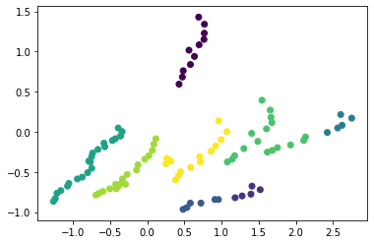
\includegraphics[width=\linewidth]{Cluster_no_class}
		\captionof{figure}{Single linkage with 2010 data}
		\label{fig:test1}
	\end{minipage}%
	\begin{minipage}{.5\textwidth}
		\centering
		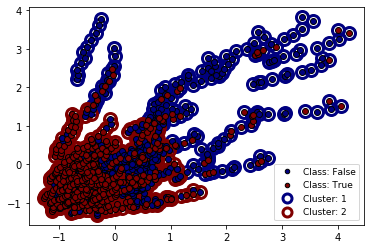
\includegraphics[width=\linewidth]{full_cluster}
		\captionof{figure}{Ward linkage with full data with target classes}
		\label{fig:test2}
	\end{minipage}
\end{figure}
\begin{figure}[H]
	\centering
	\textbf{Dendrograms based on clustering}\par\medskip
	\begin{minipage}{.5\textwidth}
		\centering
		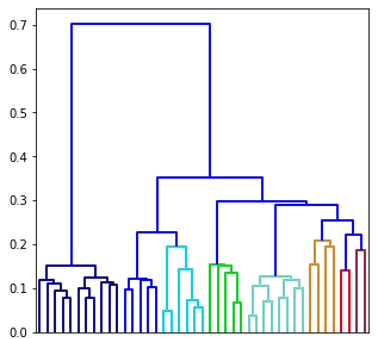
\includegraphics[width= .8\linewidth,]{Dendro_8_color}
		\captionof{figure}{Dendrogram for single linkage on 2010 data}
		\label{fig:test1}
	\end{minipage}%
	\begin{minipage}{.5\textwidth}
		\centering
		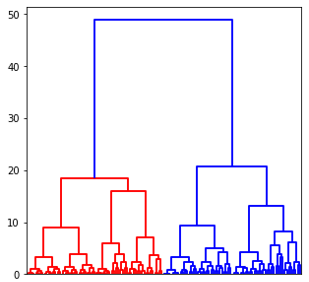
\includegraphics[width= .8\linewidth]{dendro_full_color}
		\captionof{figure}{Dendrogram for ward linkage on full data}
		\label{fig:test2}
	\end{minipage}
\end{figure}
\noindent
Though the similarity measure remained the same, namely euclidean distance, the linkage functions were changed to fit the data better.
As seen in Figure 2.2, the data from 2010, was separated clearly in quite straight lines, and therefore single linkage clustering seemed appropriate.
Single linkage is done by repeatedly clustering together the two closest clusters, when initializing every data point as a cluster, until the correct number of clusters is reached. This distance between two clusters $C_1$ and $C_2$, is then described by:
\begin{equation}
	d(C_1,C_2) = \underset{\mathbf x \in C_1, \mathbf y \in C_2}{\min} \len{\mathbf x-\mathbf y}
\end{equation}
In choosing the number of clusters, we simply counted the number of straight lines in the plot, which worked well.
In the full dataset the clusters were not as easy to distinguish between, but it was obvious that the linear nature of the data was consistent over many years.
As the target feature was binary, we choose 2 clusters for the full dataset and the Ward linkage was used.
Ward linkage is a center-based clustering method, that connects clusters based on the least squared error between the points and the centroid in a cluster. This method is inspired by the $K$-means algorithm, the precise mathematical description of which can be read in [1] (p. 297).
%\begin{equation}
%	\sum_{i = 1 }^N \sum_{k = 1 }^K z_{ik} || x_i - \mu_k ||^2_2 
%\end{equation}
As the data seemed to emanate in linear fashion from a small area around (-1.5,-1.5) we also attempted to parallel shift the data by 1.5 on each axis and use the similarity measure, cosine, as this could encapsulate the circular quality of the data. This, however, did not yield better results, and was discarded.
\subsection{Cluster types}
In \cite{skynet1} we performed PCA.
We plotted the observations in the first two latent dimensions, as shown on figure \ref{fig:PCA}.
\begin{figure}[H]
	\centering
	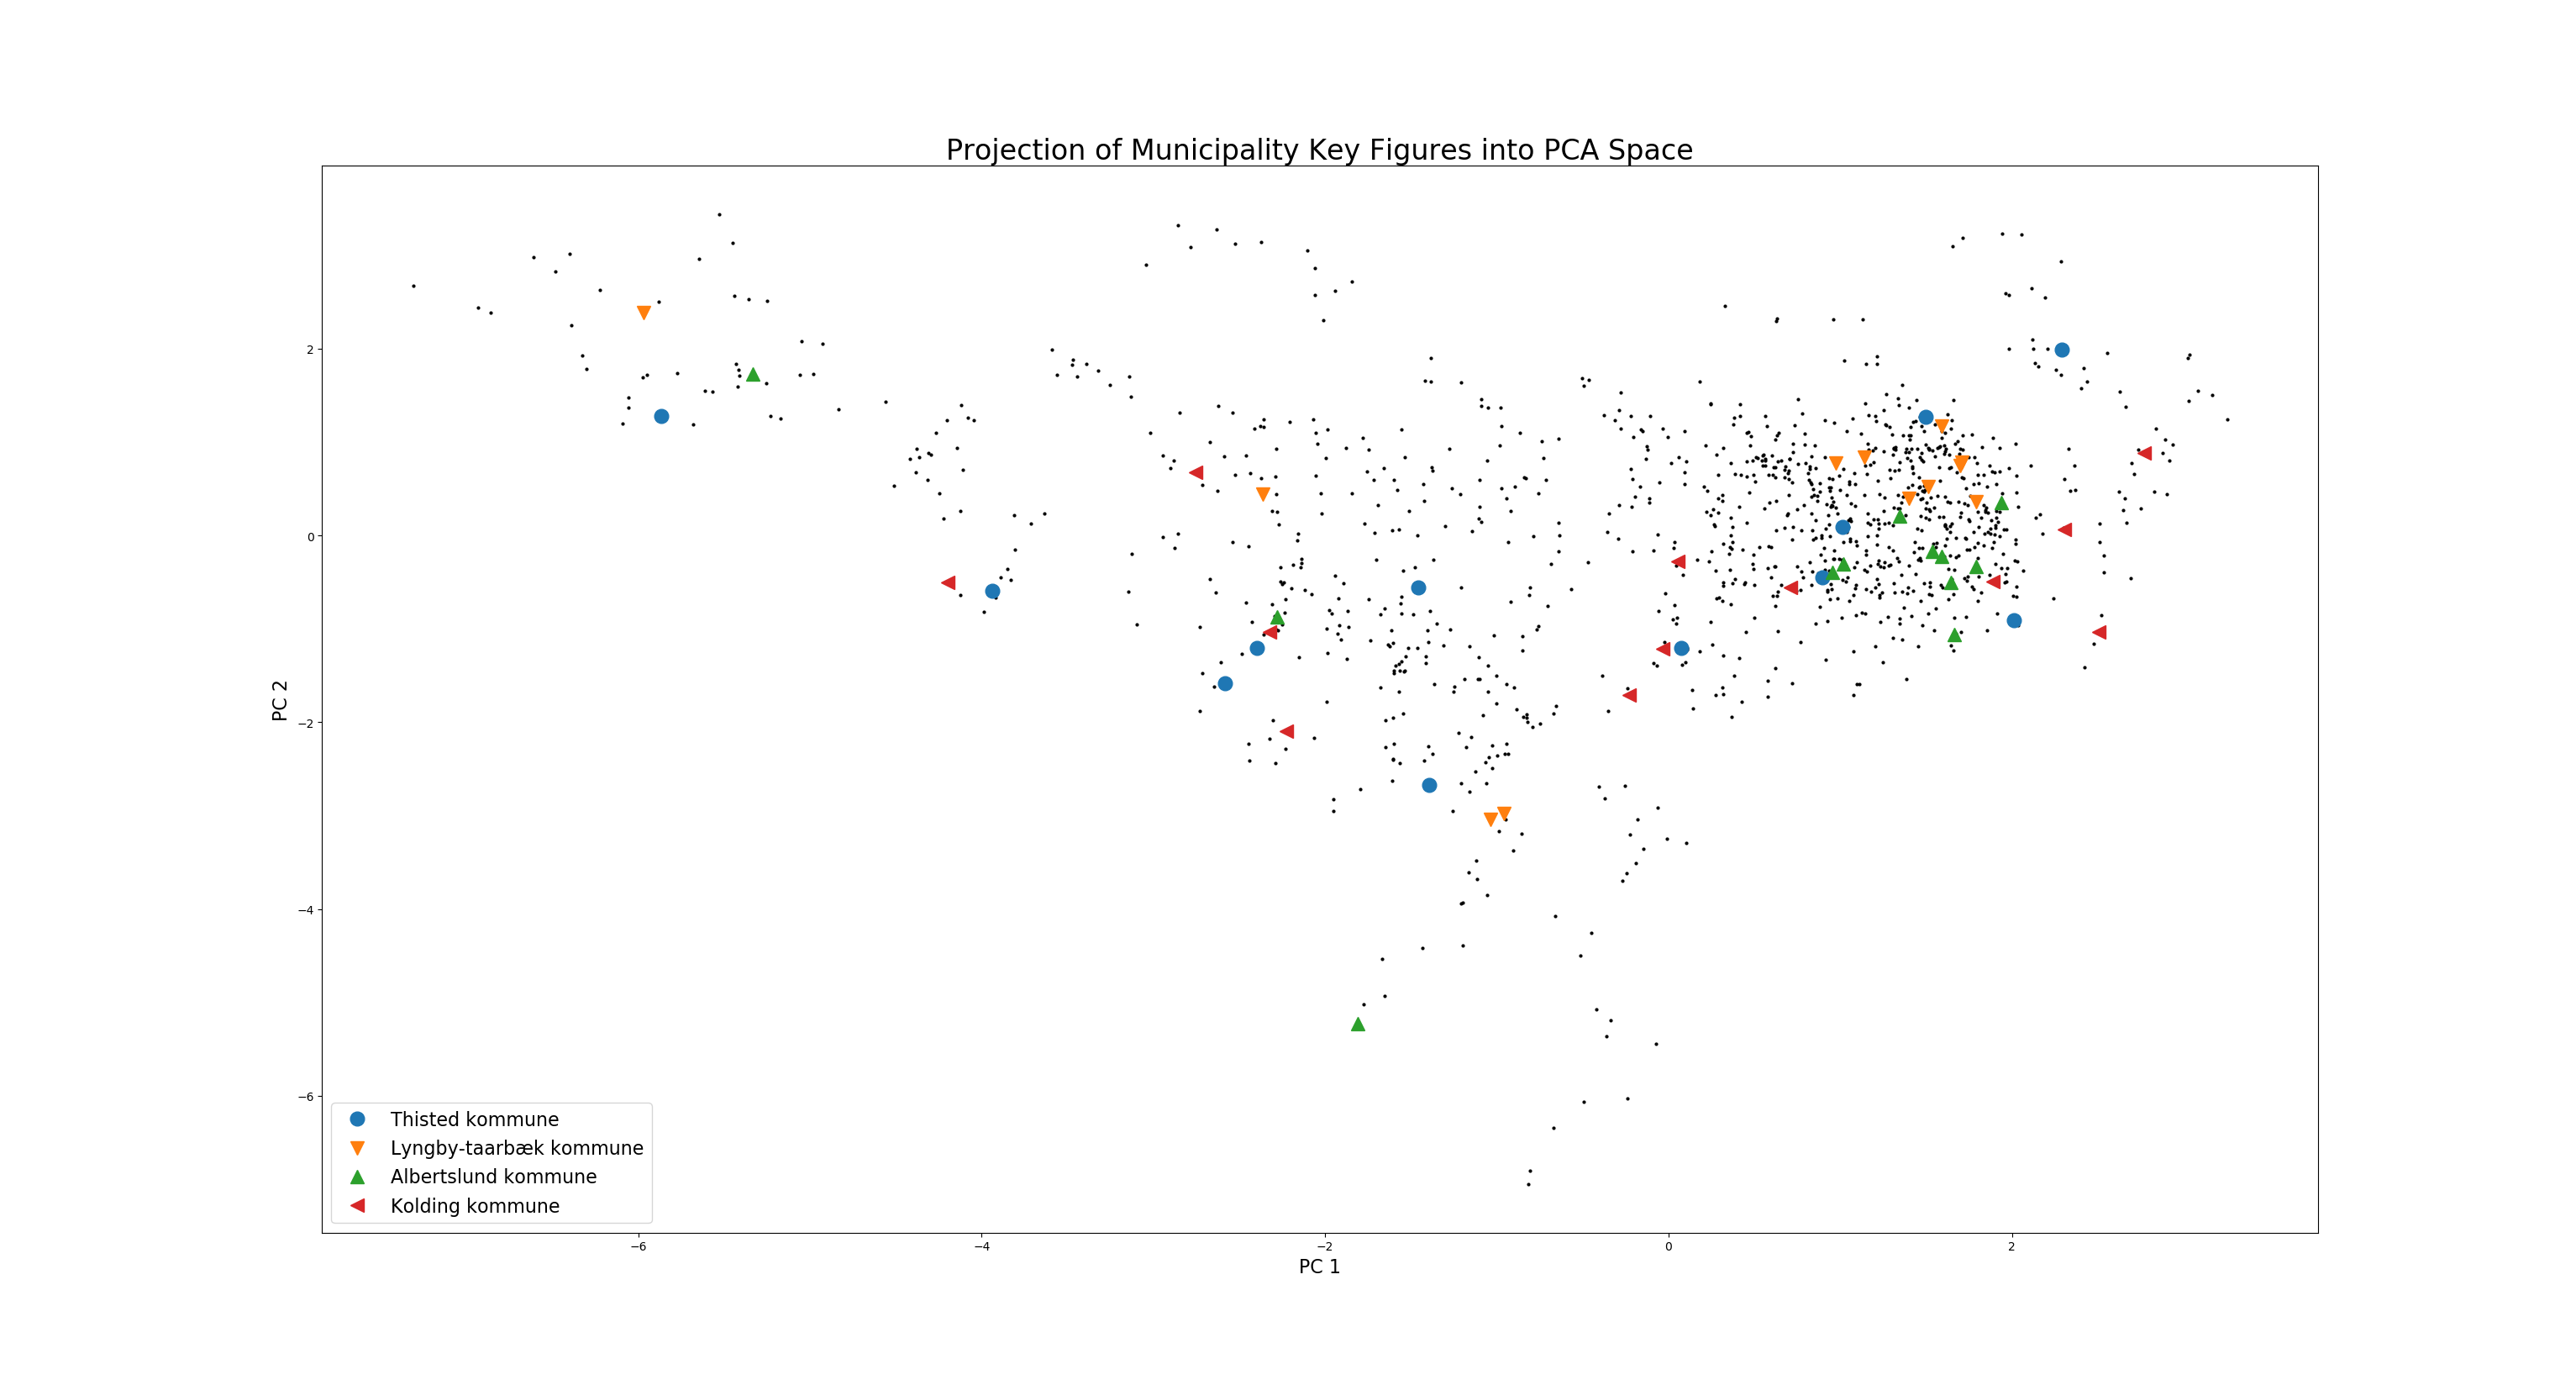
\includegraphics[width=.7\textwidth]{pca}
	\caption{The first two principal components of the dataset.}\label{fig:PCA}
\end{figure}\noindent
Figure \ref{fig:PCA} shows only the first two principal components, so some information is lost.
However, there does seem to be some clusters, even though they are rather ill-defined.
They seem to be mainly center-based, such that most points are closer to the center of their respective clusters than any other cluster centers.
This is of course not true for every point and depends on where the real clusters are, however it still gives an idea of the structure of the dataset.

\subsection{Clusting be Gaussian Mixture Model(GMM)}
As mentioned earlier, the target data was transformed into a binary set of classes depending on whether the \textbf{RT} feature was below or above mean. As such, there only existed two true labels, here named \textit{Low Risk} and \textit{High Risk}. Therefore we started out by training a Gaussian Mixture Model (GMM) with K=2 clusters using the \textit{sklearn} python library. In \textit{sklearn} the GMM implements the expectation-maximization(EM) algorithm to do the fitting of the mixture Gaussian model to get the parameters for $\mu$ (mean), $\Sigma$ (covariance matrix), and $\pi$ (weights) that best approximate the dataset.
\\
As K was set to 2 we instead made the covariance type (cv-type) the variable and created a couple of experiments just to get an idea of how the cv-type can influence accuracy when predicting clusters for the two classes of data points. Four cv-types were investigated
\begin{table}[H]
	\centering
	\begin{tabular}{|l|l|}
		\hline
		\textbf{Cv-type} & \textbf{Description} \\
		\hline
		Full & Each component has its own general covariance matrix\\
		Tied & All components share the same general covariance matrix\\
		Diag & Each component has its own diagonal covariance matrix\\
		Spherical & Each component has its own single variance\\
		\hline
	\end{tabular}
\end{table}
\noindent
\begin{figure}[H]
	\centering
	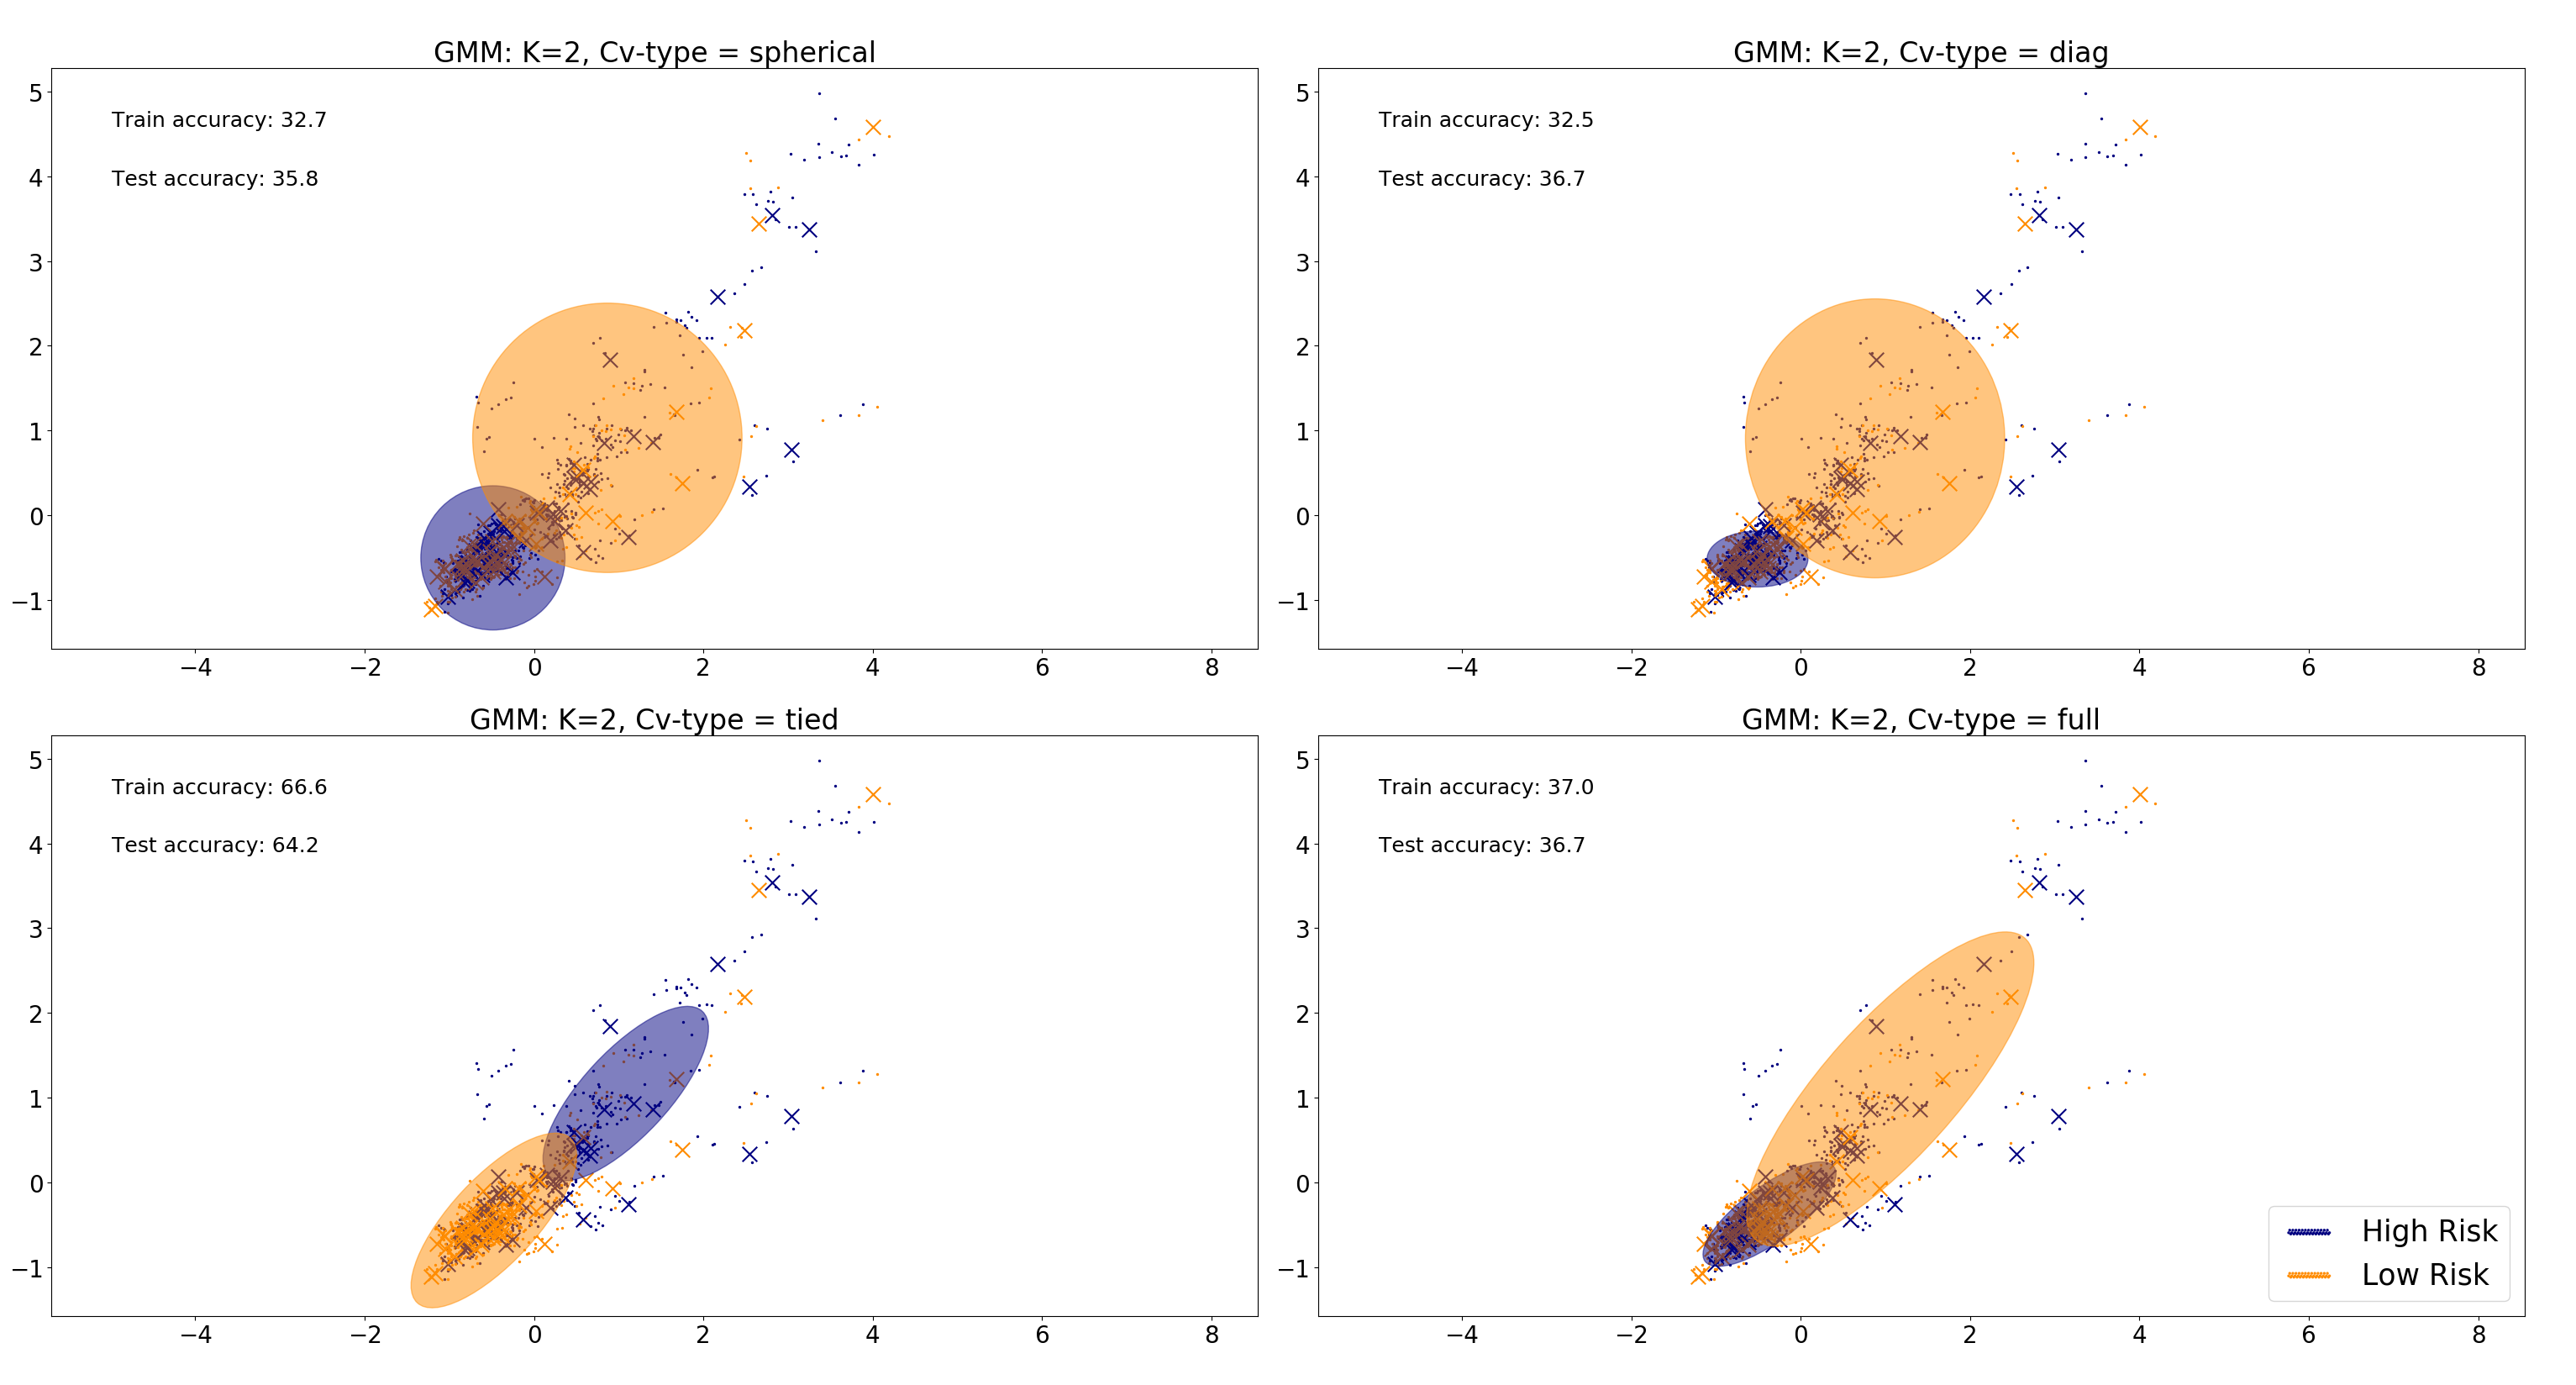
\includegraphics[width=\textwidth]{accuracy_GMM}
	\caption{Accuracy of GMM, in a single fold, based on covariance type. Test data is plotted with an 'X'}\label{fig:PCA}
\end{figure}\noindent
From the result it was possible to get an idea about the cv-type and its influence on the clustering. From the results it looked like the \textit{tied} cv-type might be worth looking into. But, this was just based on a few experiments on a couple of training and test folds, not an entire cross-validation. As mentioned earlier, these experiments were only performed to enhance our understanding of the co-variance type. To be able to actually rely on the results a thorough validation should be performed, which has not been pursued in this report. But, nonetheless the experiments points in a direction of the \textit{tied} cv-type being worth looking into for this clustering problem.
\\
Besides testing the data on two predefined clusters, we thought it interesting to investigate which number of cluster components would be chosen as the best fit for the data. For this a two-layer cross validation was used on GMMs with cv-type \textit{full} and $ K=1 $ to $ K=30 $ cluster components. The cv-type \textit{full} was used due to issues with the matrix shape when trying out the \textit{tied} cv-type.
The score of the fit was made using the negative log-likelihood
\begin{equation}
\begin{aligned} -\mathcal{L}^{\text {test }}(\boldsymbol{\pi}, \boldsymbol{\mu}, \boldsymbol{\Sigma}) &= -\log p\left(\boldsymbol{X}^{\text {test }} | \boldsymbol{\mu}, \boldsymbol{\Sigma}, \boldsymbol{\pi}\right) \\ &= -\sum_{i=1}^{N^{\text {test }}} \log \left[\sum_{k=1}^{K} \pi_{k} \mathcal{N}\left(\boldsymbol{x}_{i}^{\text {test }} | \boldsymbol{\mu}_{k}, \boldsymbol{\Sigma}_{k}\right)\right] \end{aligned}
\end{equation}
which can be computed using the negative result of the sum of the \textit{sklearn} function \textit{score\_samples} from the \textit{GaussianMixture} class.
\\
The cross-validation resulted in K=14 as the optimal number of clusters for lowering the negative log-likelihood. The resulting clusters are illustrated in the figure below.
\begin{figure}[H]
	\centering
	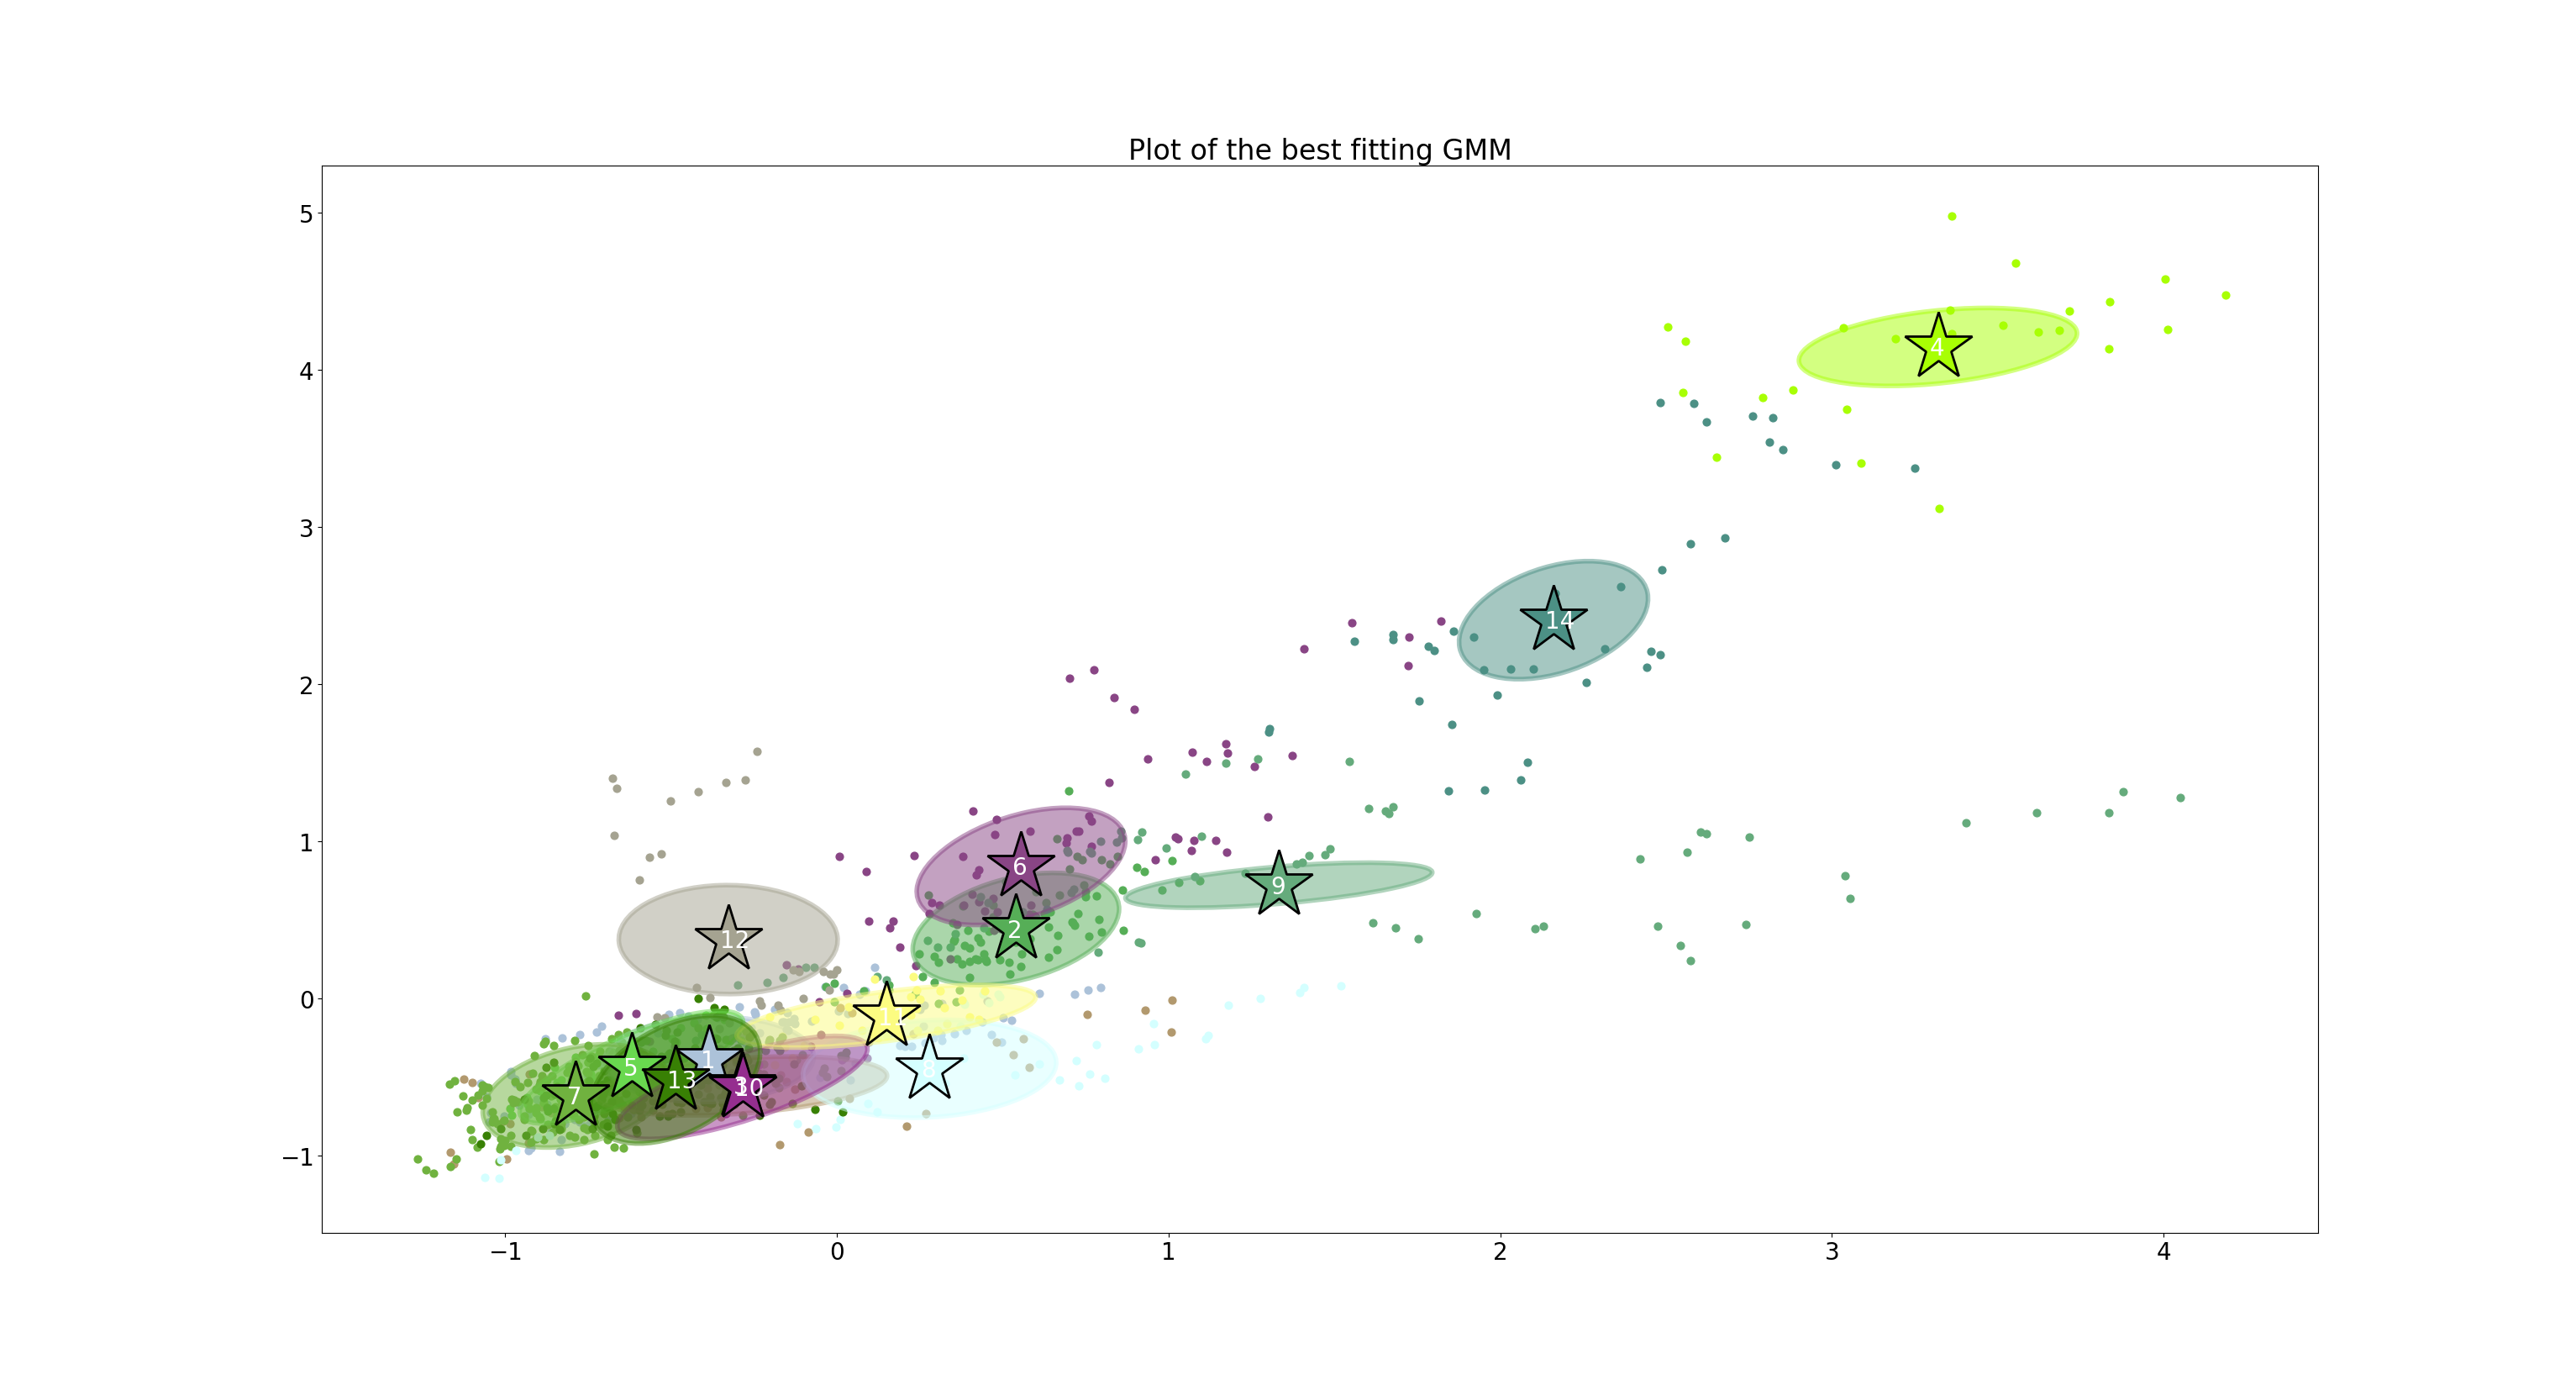
\includegraphics[width=\textwidth]{best_fitting_GMM}
	\caption{The winning GMM from nested cross validation with $ K=14 $ clusters}\label{fig:PCA}
\end{figure}\noindent
The ellipses for each Gaussian component was drawn in the eigenvector space and normalized to avoid the clusters painting over the entire plot and the data point were assigned the color of the cluster component to which they belong. The stars show the centroids of each cluster and the numbering, even though a bit off, serves the purpose of referencing the clusters in this report. Looking at the plot lower left corner, the clusters overlap a lot and end up being one big clutter. This makes it difficult to judge whether or not the clusters actually makes sense and therefore one should be careful of just accepting the GMM as a good fit for the data. On the other hand cluster 2, 6, and 9 around the middle and cluster 4, and 14 in the top right corner seems quite plausible in the way they fit the data. So from the plot it looks like 14 clusters might be a bit too many, but still there is probably a lot more groupings in the data than just the two we created in this experiment.

\subsection{Quality testing the GMM}
Now looking at the quality of the GMM according to the binary classes, we tried both a model with two clusters and the optimal with 14, just for fun. We expected the model with 14 clusters to do a very poor job, since the many classes did not match the two classes created by us. Surely, the results were bad, which can be seen in the table below:

\begin{table}[H]
	\centering
	\begin{tabular}{|l|l|}
		\hline
		\textbf{Quality Test Type} & \textbf{Score} \\
		\hline
		Rand Index Score & 0.5125658265331962\\
		Jaccard Similarity Score & 0.11132711900604264\\
		Normalized Mutual Information (NMI) Score & 0.08118995950534755\\
		\hline
	\end{tabular}
\end{table}
\noindent
The rand index score shows a similarity of approximately 51 percent, so the 14 cluster GMM only agrees with the true labels about half the time. Also, a problem that we need to be aware of here is, that when there are a lot of clusters, as in this experiment, the Rand index has a tendency to be artificially close to 1 (completely similar). This is something the Jaccard similarity score tries to avoid. And as it turns out, this score shows a lot less similarity, only about 11 percent, which is a bit more realistic. Finally the NMI tries to quantify how much information the partition provides about the other. And here we hit a bottom low with only 8 percent similarity. After all this was expected as explained earlier. We then thought it interesting to see how a $ K=2 $ GMM would perform on the data.
We tried to test it and got the following result:
\begin{figure}[H]
	\centering
	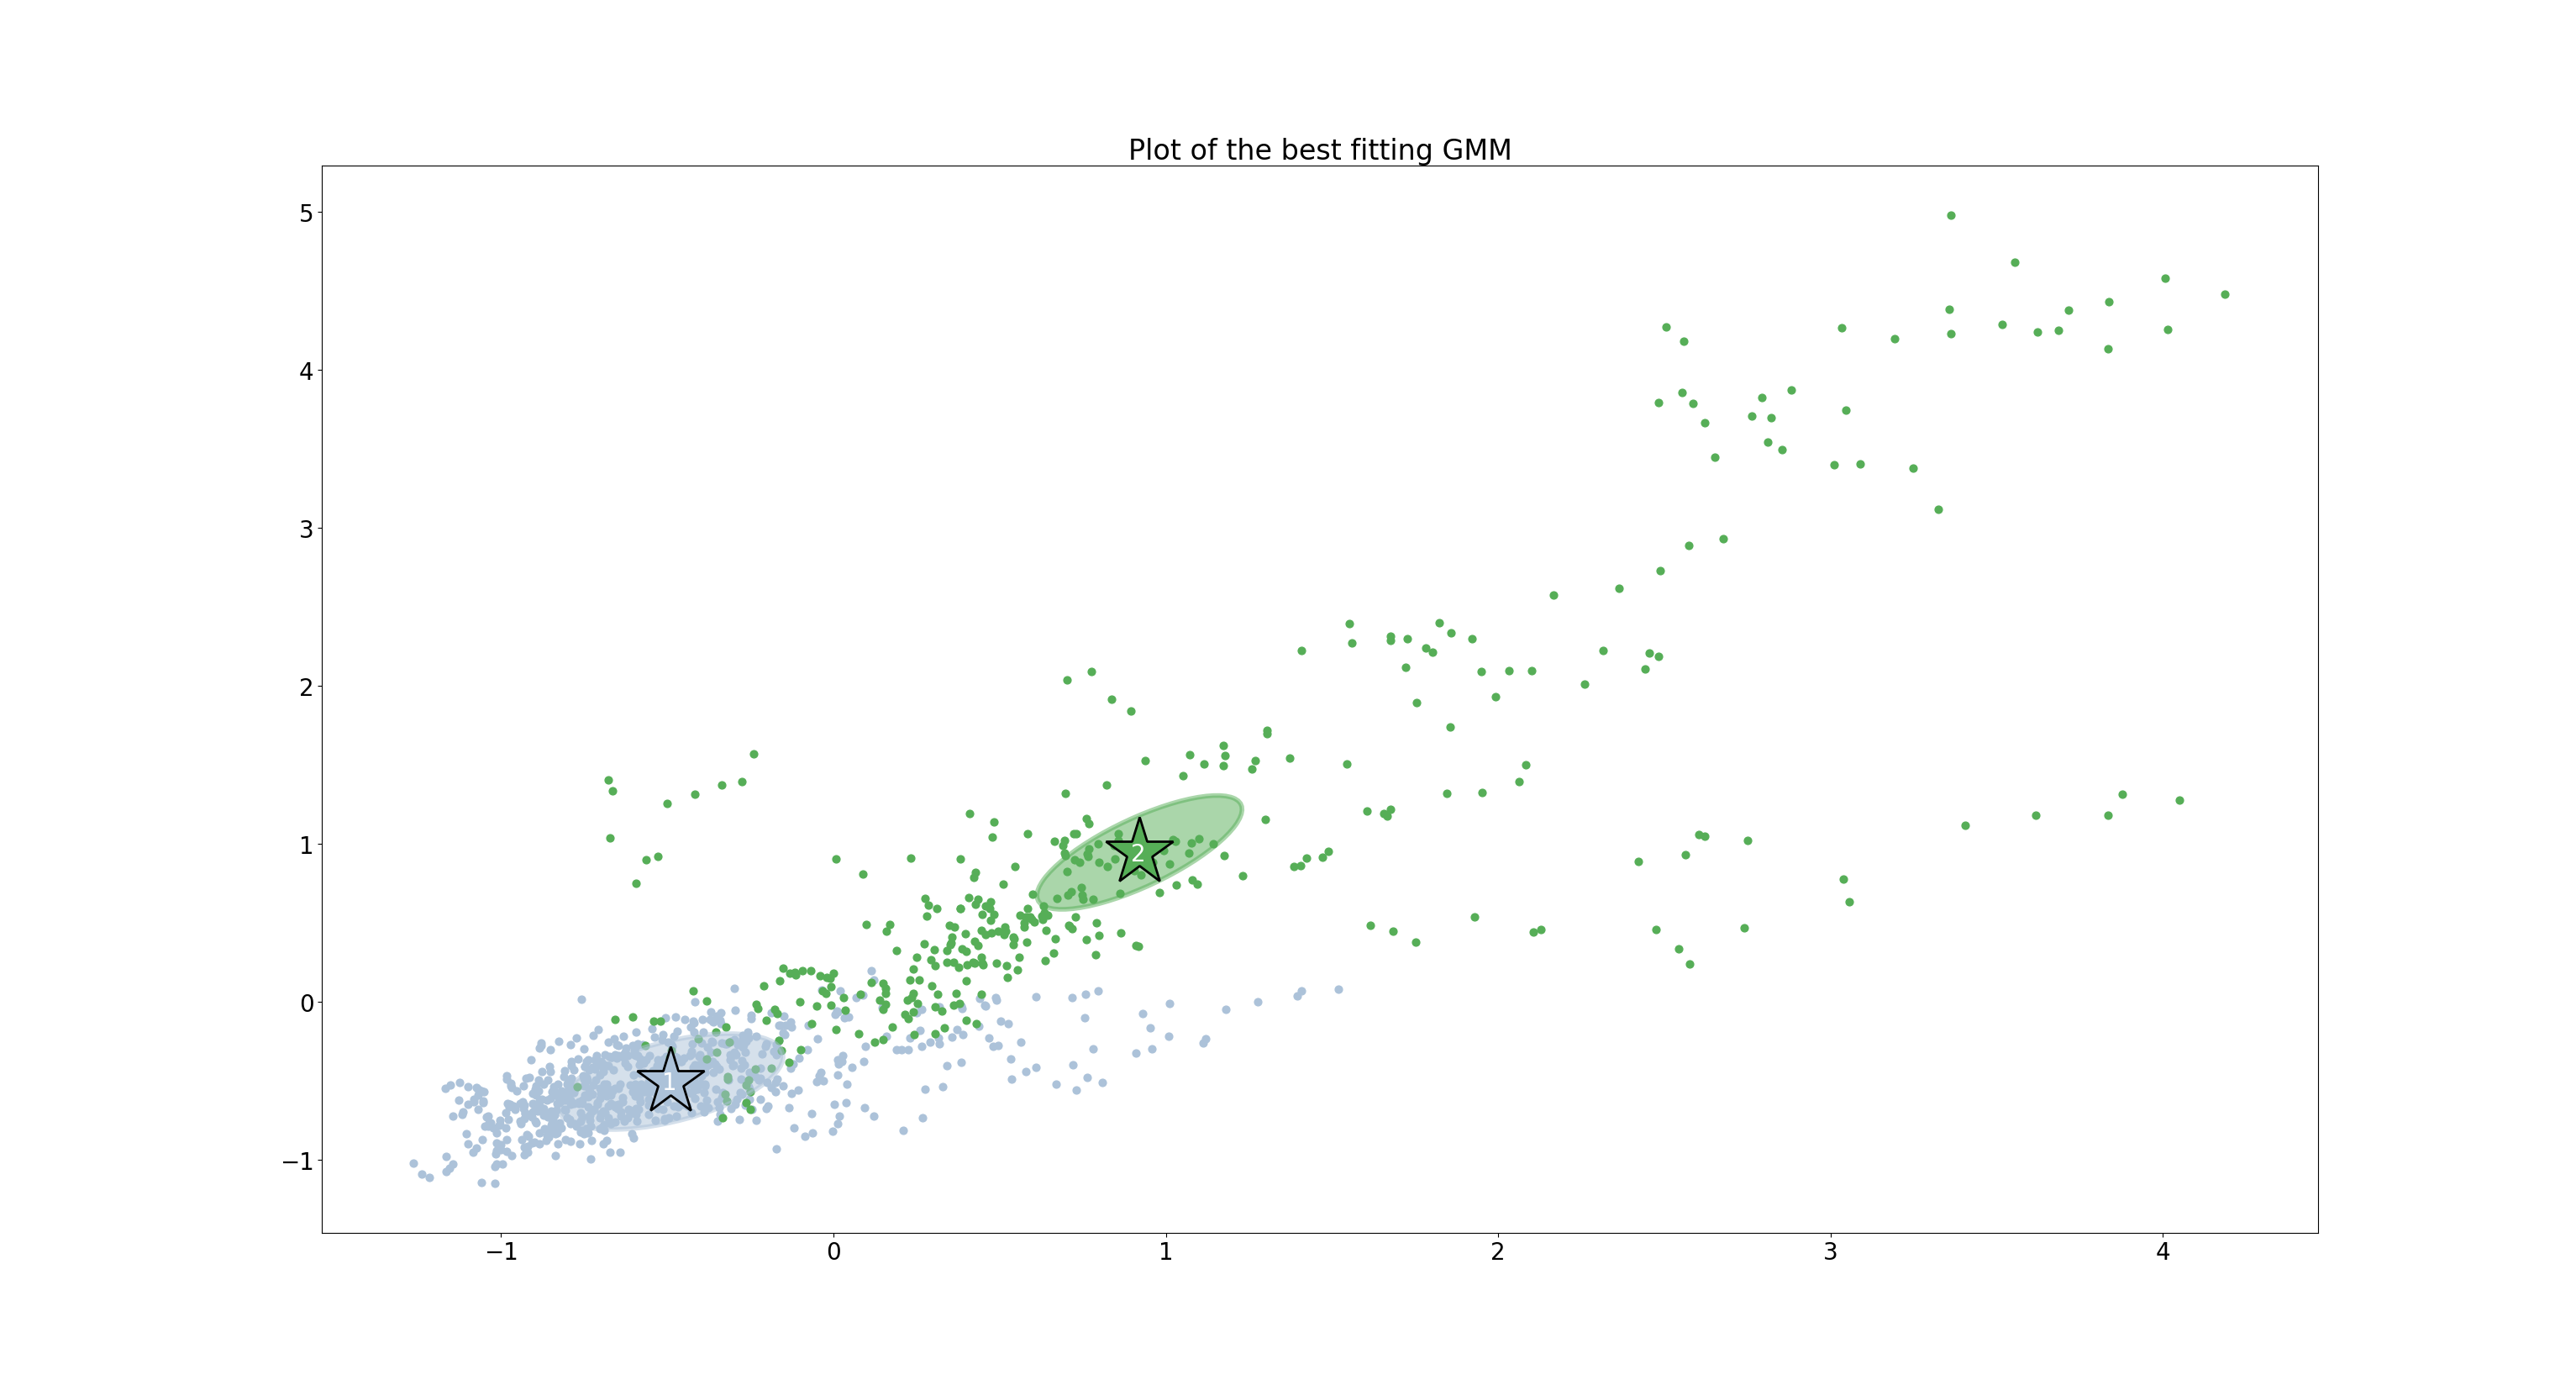
\includegraphics[width=\textwidth]{GMM_2_clusters}
	\caption{GMM $ K=2 $ clustering}\label{fig:PCA}
\end{figure}\noindent
interestingly enough the similarity scores were not that different here:
\begin{table}[H]
	\centering
	\begin{tabular}{|l|l|}
		\hline
		\textbf{Quality Test Type} & \textbf{Score} \\
		\hline
		Rand Index Score & 0.5630392952318937\\
		Jaccard Similarity Score & 0.2112678802282913\\
		Normalized Mutual Information(NMI) Score & 0.11482413218698861\\
		\hline
	\end{tabular}
\end{table}
\noindent
This all in all points to the conclusion, that the settings for the GMM might not fit that data very well, and that further experiments for tuning other parameters like the regularization constant $\lambda$ or the cv-type should be conduct. Also, it could be an option simply to try other models for the data than a GMM.

\section{Anomaly Detection}
% !TeX spellcheck = en_GB
A common issue with data are outliers or anomalies.
These are observations that do not seem to follow the same pattern as the remaining observations.
This is often due to measurement errors, but it could also be due to a more complex relationship between (potentially hidden) features, so one must be careful about removing data, even if it seems out of place.
Here three methods of detecting outliers will be explored.

\paragraph{Gaussian Kernel Density (GKD/KDE)}
This method produces a multivariate distribution around each observation with a mean the observation's value and a standard deviation $ \lambda $.
Leave-one-out cross-validation is then performed -- leaving each observation out and calculating the sum of all other observations' density functions (usually with a logarithm applied for numerical stability).
This produces estimates of the likelihood that observations fit with the rest of the dataset.\\
\\
For this method to be applicable, $ \lambda $ must be known.
This is found using brute force.
For a range of $ \lambda $'s, in our 21 log-spaced points from $ -6 $ to 1, the mean of all $ \log $ likelihoods is calculated.
The $ \lambda $ with the highest mean log probability was then selected.
We found $ \lambda=0.1778 $ to be the best.
The log probability for different $ \lambda $'s can be seen on figure \ref{fig:lambdas}.
Not all values are shown, as low values of $ \lambda $ led to values so low that taking the log would result in a number too low for the 11 exponent bits in 64 bit floating point numbers to represent.\footnote{https://floating-point-gui.de/formats/fp/}
\begin{figure}[H]
	\centering
	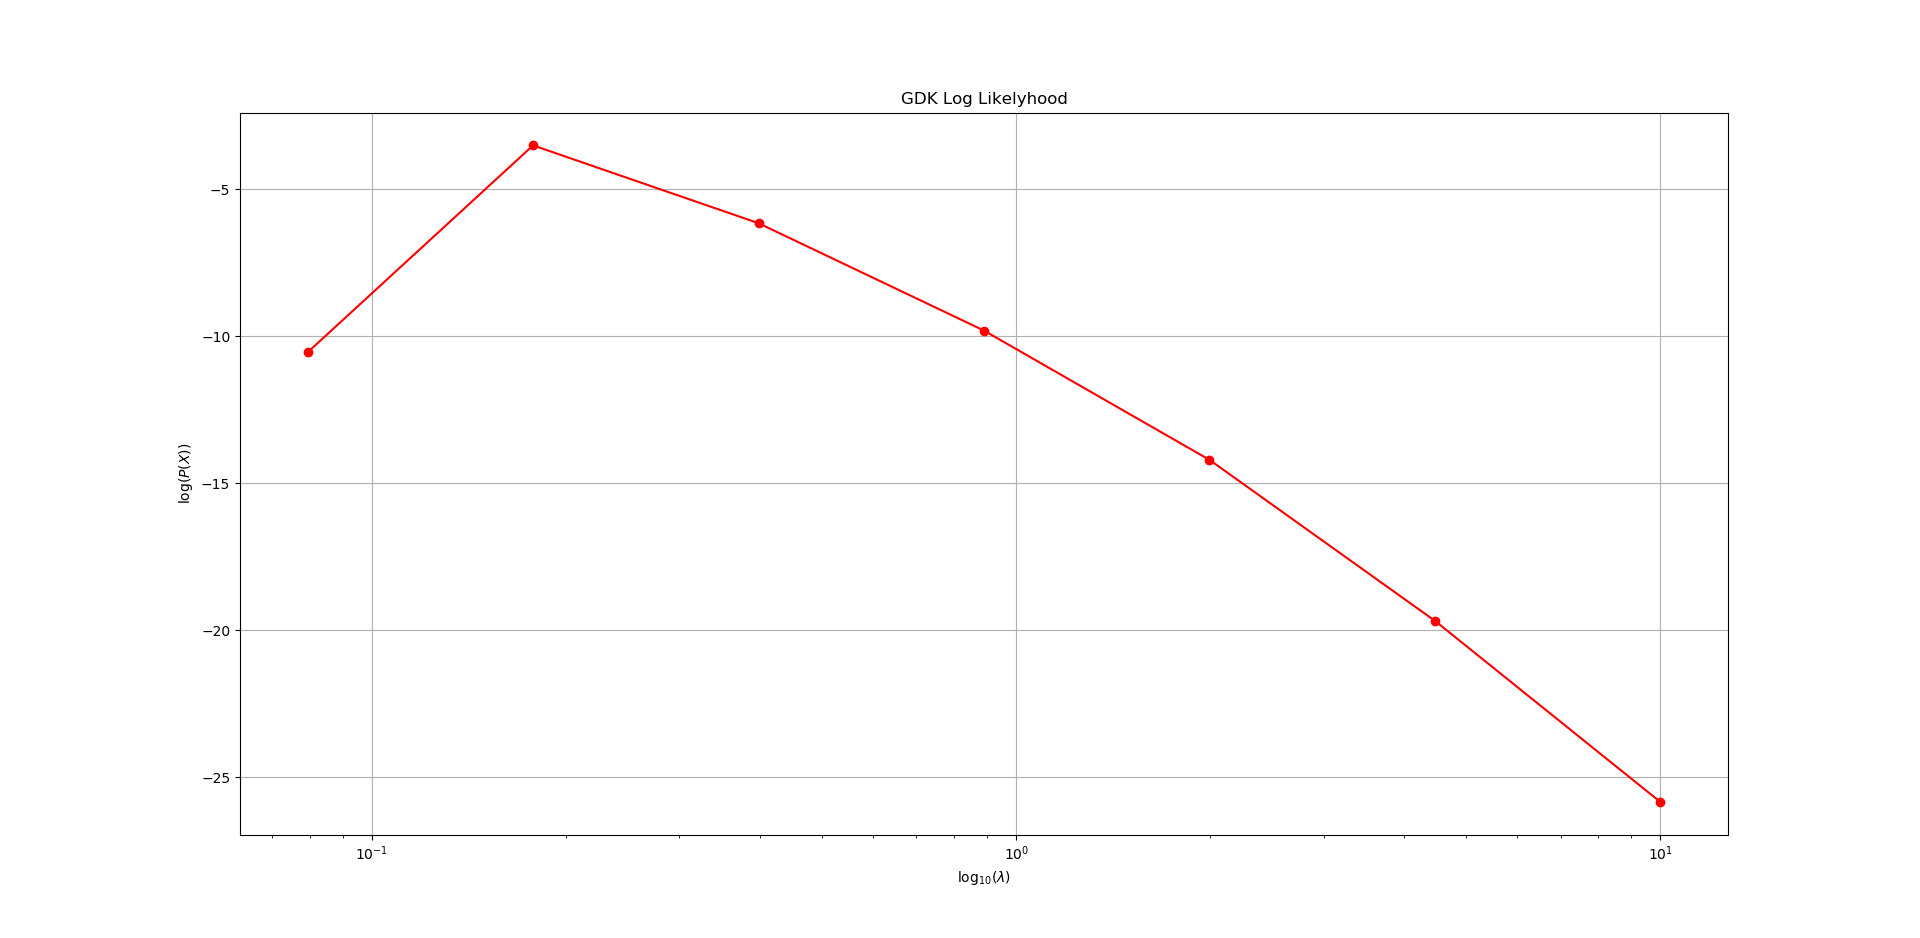
\includegraphics[width=.7\textwidth]{gdk}
	\caption{Mean log probabilities for different values of $ \lambda $.}
	\label{fig:lambdas}
\end{figure}\noindent

\paragraph{KNN Density (KNNDE)}
This method looks at the $ K $ nearest neighbours to a given observation and determines the density this way. We selected $ K=10 $ based on preliminary testing.
The density is then calculated as
\begin{equation*}
	\operatorname{density}_{\mathbf X}(x, K)=\frac{K}{\sum_{x'\in N_{x, K}}d(x, x')}, \quad d=\len{x-x'}
\end{equation*}
This method works well in many cases, but it has one major drawback, which the next method aims to solve.

\paragraph{KNN Average Relative Density (ARD)}
This method takes into account clusters of different densities such that dense clusters do not dominate as much, which is a major improvement over GDK and KNNDE.
It is build on KNNDE and calculated as
\begin{equation*}
	\operatorname{ard}_{\mathbf X}(x, K)=\frac{K\operatorname{density}_{\mathbf X}(x, K)}{\sum_{x_j \in N_{\mathbf X}}(x, K)\operatorname{density}_{\mathbf X_{\backslash j}}(x_j, K)}
\end{equation*}
Again, we used $ K=10 $.

\paragraph{Comparison}
We ranked all observations according to the different methods described. The results are shown on figure \eqref{fig:ting}.
\begin{figure}[H]
	\centering
	\begin{minipage}[t]{.3\textwidth}
		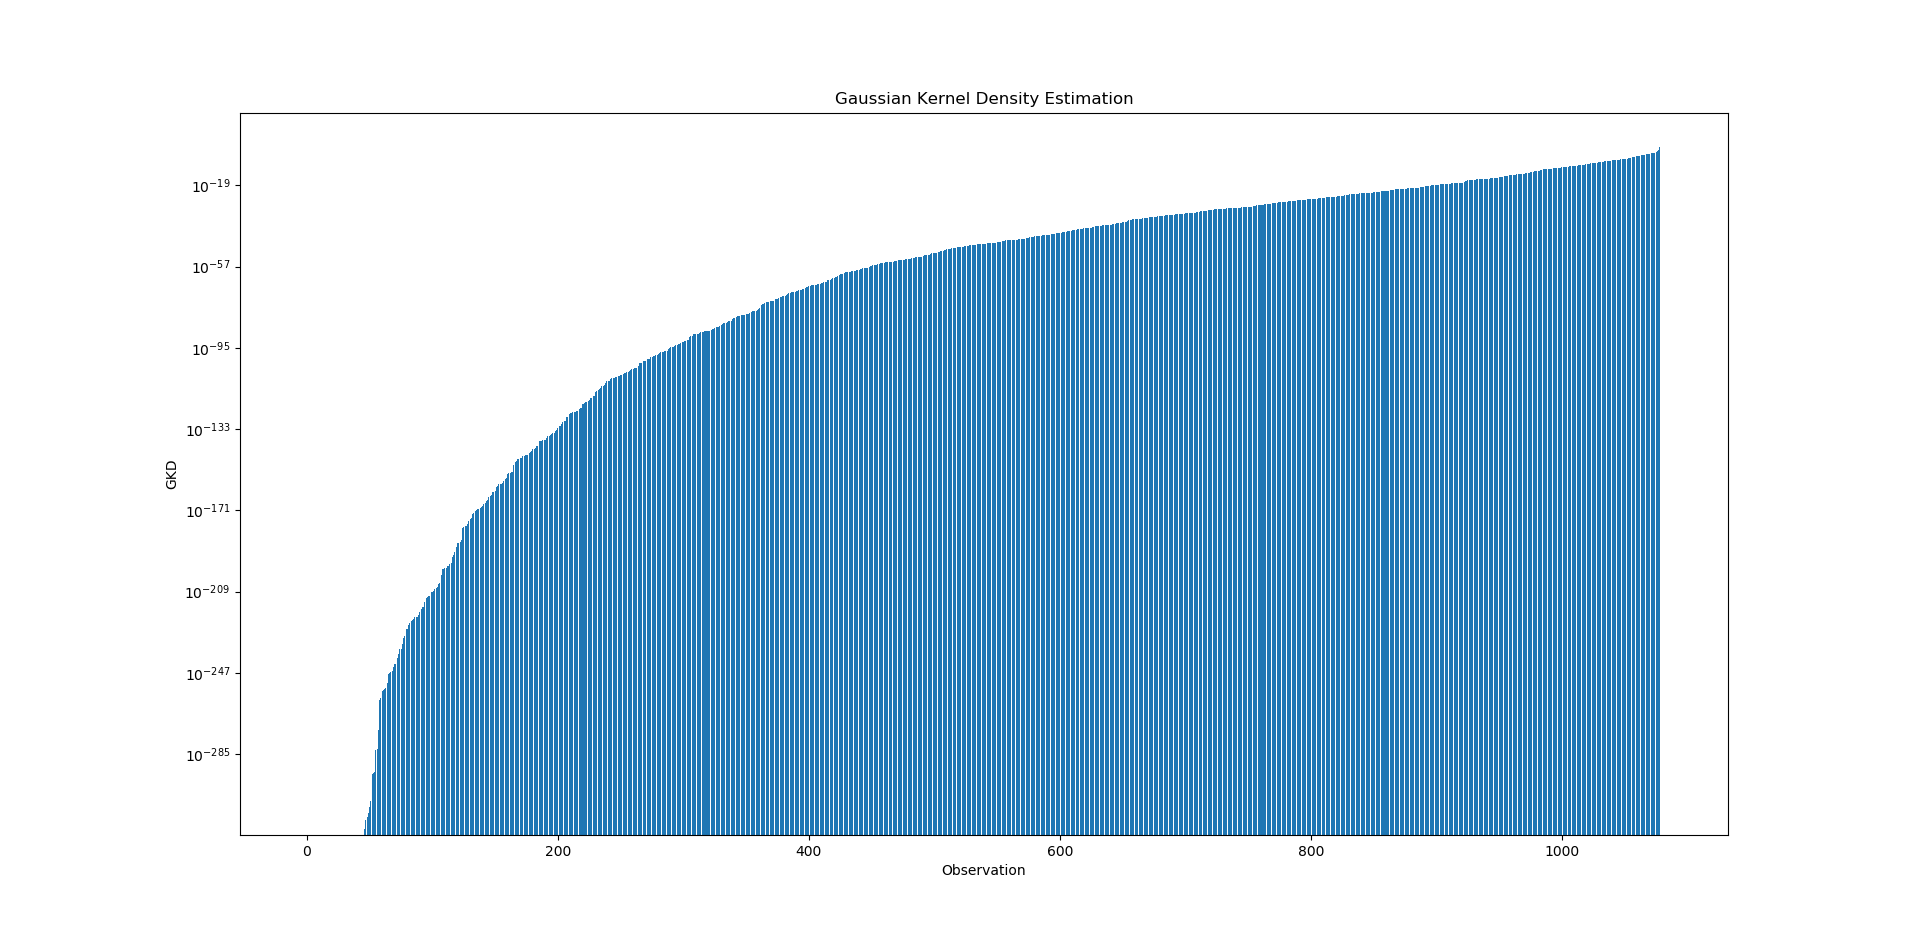
\includegraphics[width=\textwidth]{gdk-ll}
	\end{minipage}\hfill
	\begin{minipage}[t]{.3\textwidth}
		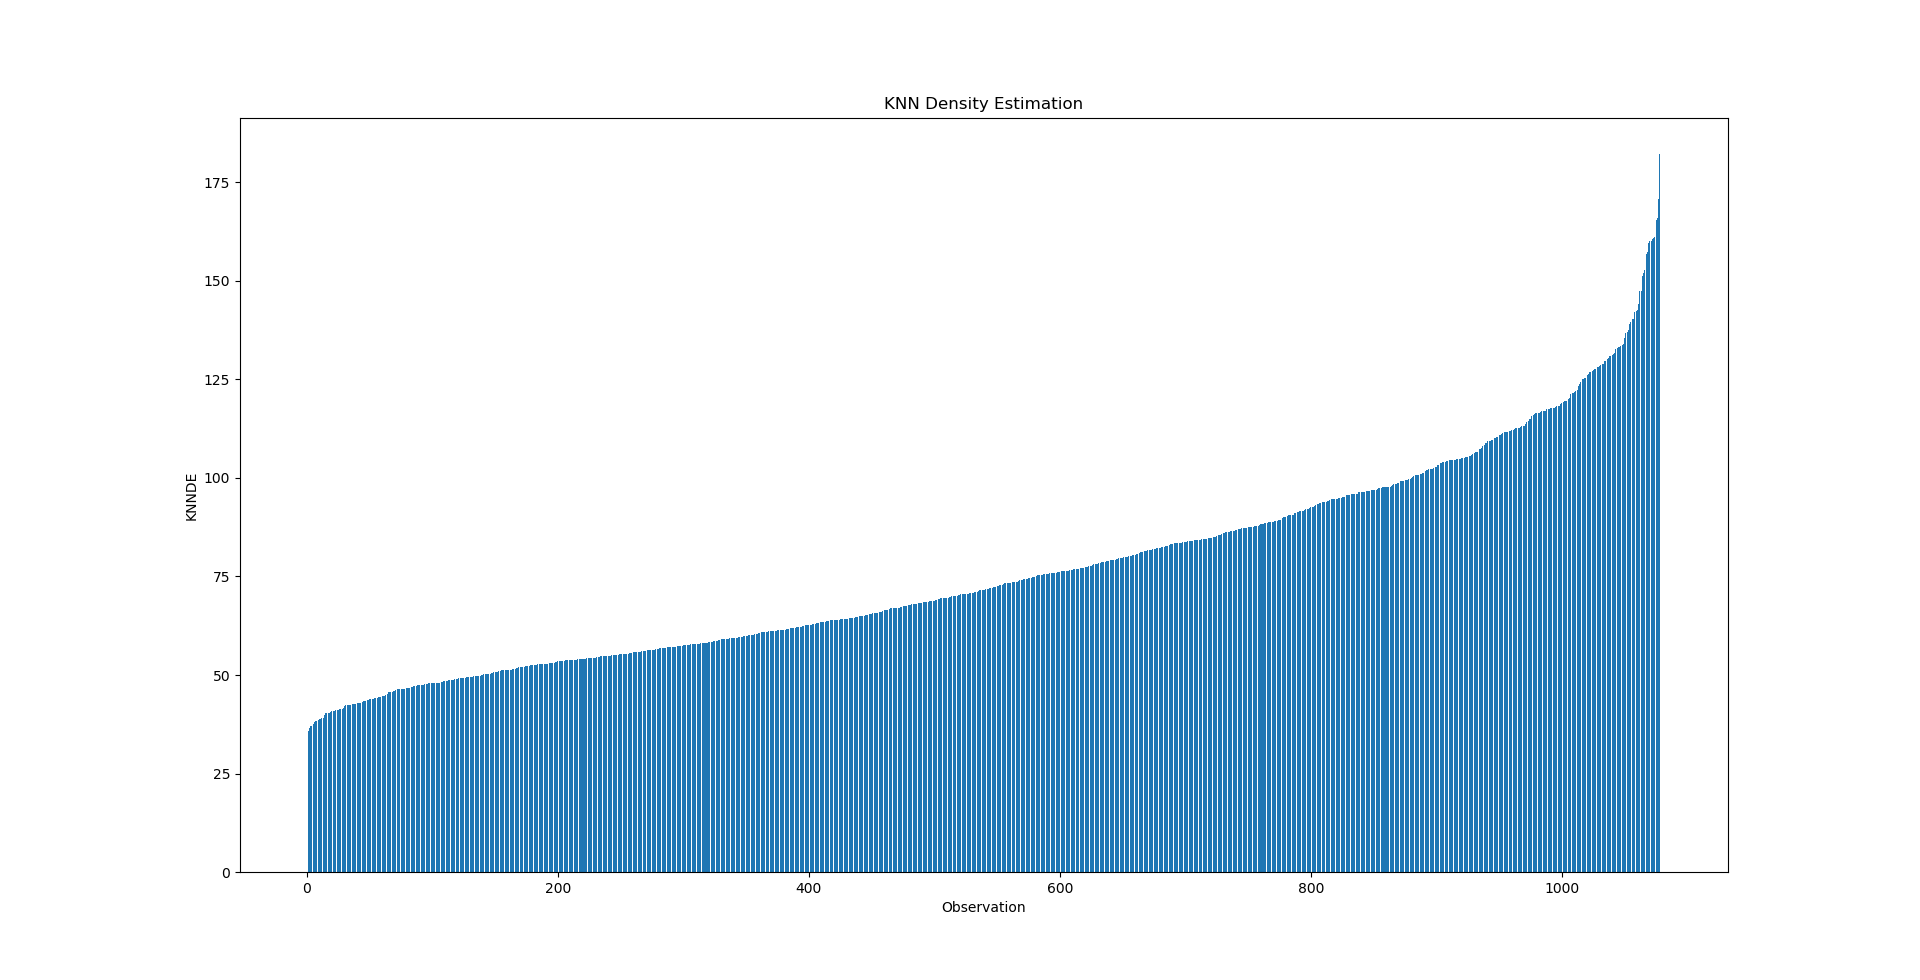
\includegraphics[width=\textwidth]{kde}
	\end{minipage}\hfill
	\begin{minipage}[t]{.3\textwidth}
		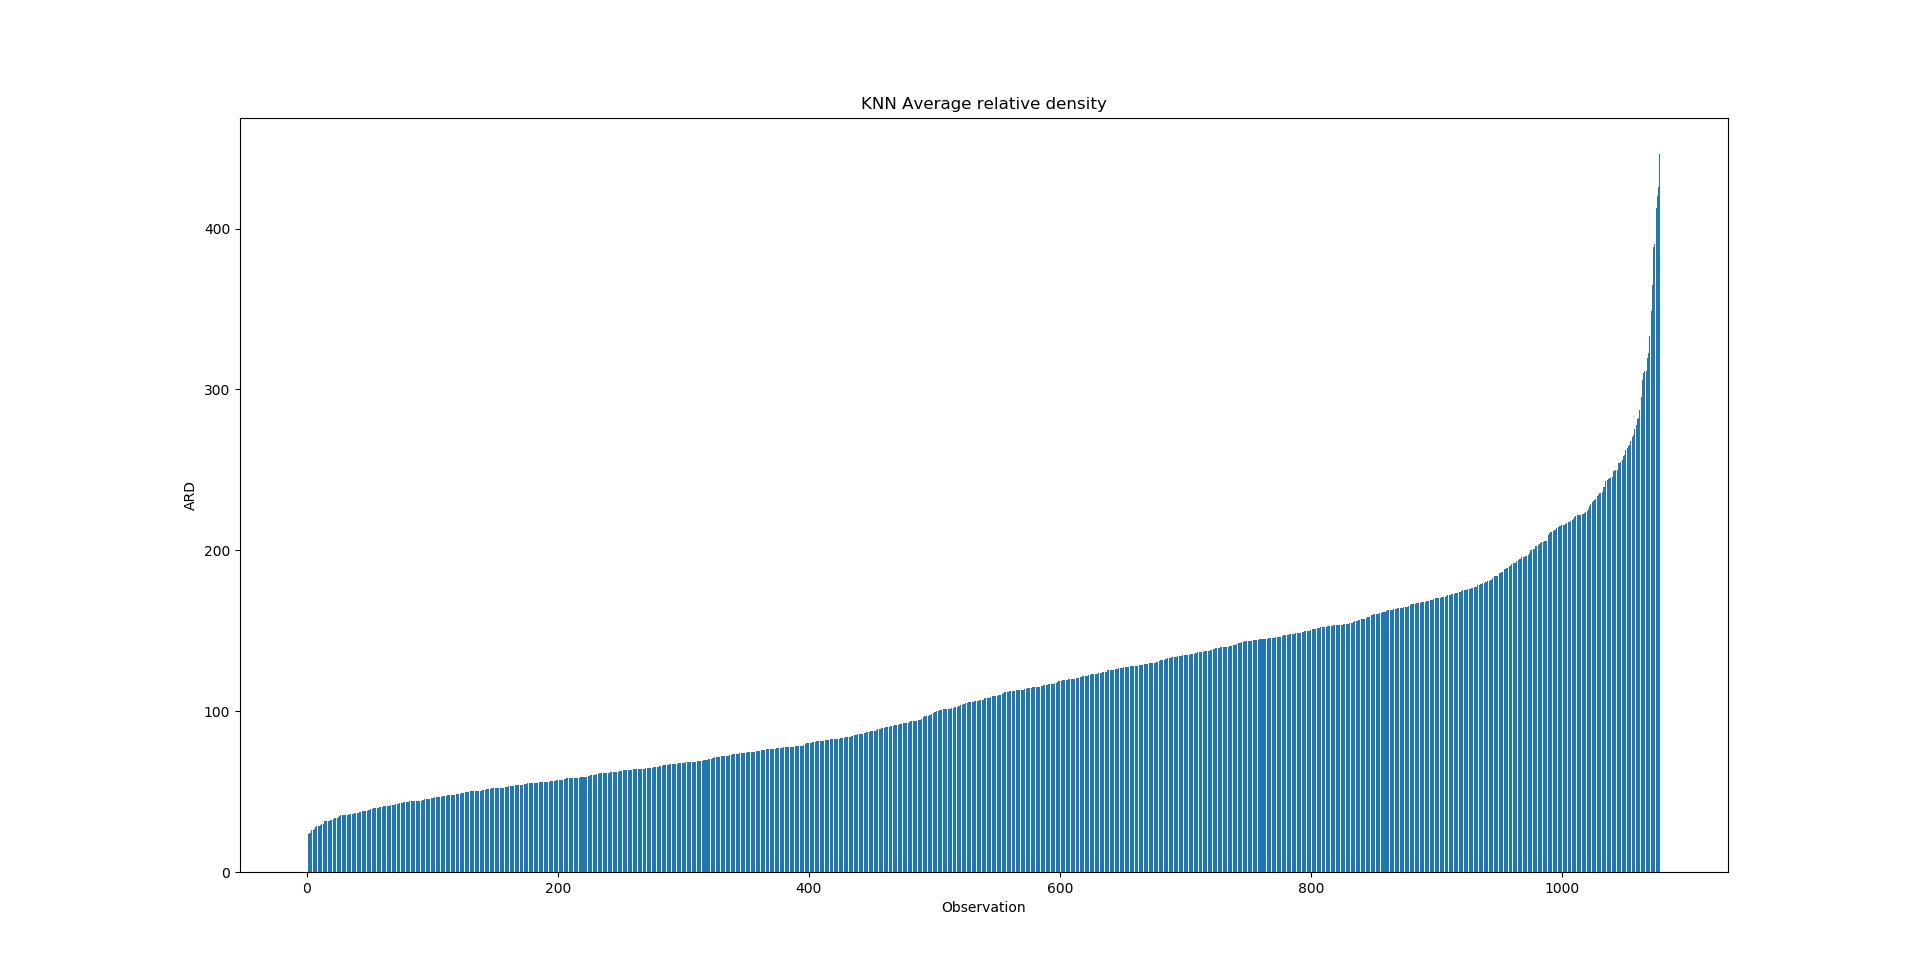
\includegraphics[width=\textwidth]{ard}
	\end{minipage}\hfill
	\caption{Outlier scoring with different methods.}\label{fig:ting}
\end{figure}\noindent
We opted to use a log scale for GKD as the values varied greatly.
GKD disagrees quite a bit with the remaining models, as it predicts a good chunk of the dataset to be outliers, whereas the other two methods show no clear outliers.
















\section{Association Mining}
Association mining was done on the 8 attributes, with the apriori algorithm.
The support was set very low, at 0.25, with a confidence of 0.6, to give any rules.
The 3 rules with highest support, two of which were mutually dependent, are listed below: \\
R1: GD $ \rightarrow $ PS  (supp: 0.288, conf: 0.651)
(PS $ \rightarrow $ GD  (supp: 0.288, conf: 0.620) ) \\
R2: JA $ \rightarrow $ VE  (supp: 0.288, conf: 0.611)  \\
R3: NW $ \rightarrow $ GD  (supp: 0.278, conf: 0.713) (GD $ \rightarrow $ NW  (supp: 0.278, conf: 0.628) ) \\
Rule 1 and 3 suggests that if a municipality has above mean Gross Daycare expenses, this municipality will also have above mean expenses towards Public primary School and more citizens from Non-Western countries (and the other way around with both). The first rule is quite logical, as a municipality with a high number of children, would benefit from both high expenses towards daycare and primary school in no specifik order. On top of that, any preference among citizens and politicians for high expenses in one field would likely result in the same preference for the other. Why an above mean number of non-western citizens is accompanied above mean daycare expenses is not as easy to interpret, but could be explained by non-western women having more children than women born in Denmark\footnote{https://www.dst.dk/Site/Dst/Udgivelser/nyt/GetPdf.aspx?cid=28498}.\\
According to rule 2, high expenses towards Job Activation is followed by a bigger share of 25-64 year-olds without Vocational Education. This is compatible with the idea that higher education generally leads to easier employment and vice versa. High expenses in job activation could naturally be a consequence of low employment rates.

\section{Discussion}
One of the first things we discovered using clustering was that our data did not work too well with clustering, as there is often no clearly separated clusters. Furthermore, because all features were continuous, our chosen target classes were rather arbitrary.
\\\\
Looking at the clustering using Gaussian Mixture Models, the results indicate that even though we have chosen a binary classification of our data, as below and above mean \textbf{RT}, the data might consists of more classes than just those two. This seems like a fair point, as we could probably imagine municipality burglary ratings (\textbf{RT}) to be distributed in smaller groups across a spectrum rather than just two fit neatly into two boxes above and below the mean. For the sake of this report the harsh split at the mean did the job. But, was this report to be taken any further it  would demand an investigation of multiple possible groups, maybe using the clusters identified by the GMM in this report as a starting point.
\\
Also, the report found that the cv-type of the GMM could be worth looking into. During the work, we found that changing the cv-type led to changes in the shape of the covariance matrix, which brought with it new challenges when performing the matrix calculations. Therefore, due to the scope of the report and a time limit, we chose to leave this extra work as a possible future investigation.
\\
The quality evaluations of the GMM all showed that the GMM did a fairly poor job of clustering the data according to the binary labels, that we provided. This might be the model parameters, that could be tuned even better or the quality of the data. Also, part of the reason could most likely be, that the labelling into binary classes done by us is not a great fit for the data. As explained above, a binary view on the municipality data might be to simplistic and we maybe should have tried to make more classes instead.
\\\\
With regards to anomaly detection, we found that Gaussian Kernel Density Estimation found quite a lot of significant outliers, whereas the two other methods tested produced no significant outliers. This indicates that, at least in this case, the KDE method is more aggressive. Arguably the ARD method is the best -- in theory for one thing, but also because it seems to fit very well with figure \ref{fig:PCA}. No exceptional outliers, yet lots of observations could still be considered well outside a cluster.

\clearpage
\begin{thebibliography}{9}
	\bibitem{bog} Herlau, Tue et al.: "Introduction to Machine Learning and Data Mining", version 1.3.
	\bibitem{skynet1} Schultz, Asger et al.: "Feature Extraction and Visualization"\\
	Available at: \code{https://gitlab.gbar.dtu.dk/s183912/skynet}
	\bibitem{skynet2} Schultz, Asger et al.: "Supervised Learning: Classification and Regression"\\
	Available at: \code{https://gitlab.gbar.dtu.dk/s183912/skynet-2}
\end{thebibliography}

\appendix
\section{Chosen attributes}\label{app:attrs}
For this report we used the following features from the dataset:
\begin{itemize}
	\item[-] (RT) Anmeldte tyverier/indbrud pr. 1.000 indb. (Reported thefts/burglaries per 1,000 inhabitants)
	\item[-] (PV) Grundværdier pr. indb. (Property values per inhabitant)
	\item[-] (TA) Beskatningsgrundlag pr. indb. (Taxable amount per inhabitant)
	\item[-] (GD) Udg. (brutto) til dagtilbud pr. indb. (Gross daycare expenses per inhabitant)
	\item[-] (VE) Andel 25-64-årige uden erhvervsuddannelse (Share of 25-64 year-olds without vocational education)
	\item[-] (TE) Andel 25-64-årige med videregående uddannelse (Share of 25-64 year-olds with tertiary education)
	\item[-] (PS) Udg. til folkeskoleområdet pr. indb. (Expenses towards public primary school per inhabitant)
	\item[-] (NW) Statsborgere fra ikke-vestlige lande pr. 10.000 indb. (Citizens from non-western countries per 10,000 inhabitants)
	\item[-] (JA) Udg. til aktivering pr. 17-64/66-årig (Expenses towards job activation per 17-64/66 year-old)
\end{itemize}


\end{document}
